55. \begin{figure}[ht!]
\center{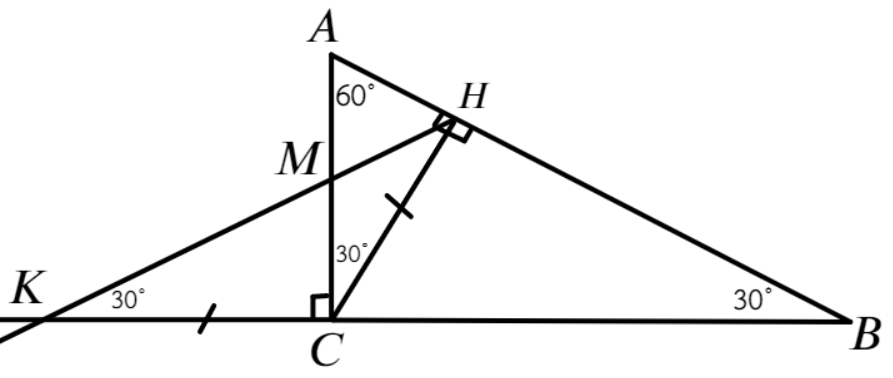
\includegraphics[scale=0.35]{g55.png}}
\end{figure}\\
Раз угол $B$ равен $30^\circ,$ угол $A$ равен $90^\circ-30^\circ=60^\circ$ и $\angle ACH=90^\circ-60^\circ=30^\circ.$  Треугольник $KHC$ является равнобедренным с углом при вершине $90^\circ+30^\circ=120^\circ$, значит $\angle KHC=\angle HKC=(180^\circ-120^\circ):2=30^\circ.$ Тогда $\angle AHM=90^\circ-30^\circ=60^\circ,$ а значит этот треугольник является равносторонним и $AH=AM=MH.$ Треугольник $MCH$ является равнобедренным, так как $\angle MCH=\angle MHC=30^\circ,$ значит $MC=MH.$  По теореме о катете, лежащем напротив угла в $30^\circ$ для треугольника $KMC$ имеем $KM=2MC.$ В треугольнике $KHB$ углы при стороне $KB$ равны по $30^\circ,$ значит он равнобедренный и  $BH=KH=KM+MH=2MC+MC=3MC.$ Таким образом, $BH:KM=3MC:2MC=3:2.$\\
